\documentclass{article}
\usepackage{listings}
\usepackage{amsmath}
\usepackage{graphicx}
\usepackage{float}
\usepackage{subcaption}
\usepackage[linewidth=1pt]{mdframed}
\usepackage[colorlinks]{hyperref}

\hypersetup{citecolor=DeepPink4}
\hypersetup{linkcolor=DarkRed}
\hypersetup{urlcolor=Blue}

\usepackage{cleveref}

\setlength{\parindent}{1em}
\setlength{\parskip}{1em}
\renewcommand{\baselinestretch}{1.0}

\begin{document}

\begin{titlepage}
	\centering
	{\scshape\LARGE Automatic code generator for matrix multiplication \par}
	\vspace{1cm}
	{\scshape\Large EAS520/DSC 520/MTH 499\par}
	\vspace{1.5cm}
	{\Large\itshape Sri Kanya Mullapudi, Dwyer Deighan, Javier Arechalde\par}
	\vfill
	{\large \today\par}
\end{titlepage}

\section*{1. Introduction}

Automatic programming is a type of computer programming which consists of some mechanism that generates computer code or program to allow programmers or users to write code at a higher level. Automatic programming has been a really useful tool, as it has allowed programmers to save a lot of time, by automating, or simplifying repetitive tasks. There are several different types of automatic programming, here we will list the most common ones:

\begin{enumerate}
 \item{\textbf{Generative programming:}}
 Generative programming is a type of computer programming that creates source code to help programmers save time, thanks to code reusing.
 \item{\textbf{Source code generation:}}
 Source code generation tools allow the generation of source code based on an ontological model such as a template, and is accomplished with a programming tool such a template procesor or an IDE \textit{(Integrated Development Enviroment)}.
 \item{\textbf{Low code aplication:}}
 This type of automatic programming, consists on tools that simplify the development of applications for rapid development. This tools usually are higher level tools that simplify other complex tasks in example: user interface creation, web development, etc.
\end{enumerate}

The purpose of this project is to develop a code generation tool, in this specific case, a source-to-source compiler, to help speed up matrix multiplication on Python. We will accomplish this by generating and compiling C code in a Python script. This tool will consist of a template-like code in Python, that will take two matrices as its input, and it will dynamically generate C code to compute the matrix multiplication in C.

The speed up can be accomplished thanks to C being a programming language rather than a scripting language like Python. Scripting languages, are interpreted and executed at the same time, while programmed languages are interpreted or compiled once and then executed whenever required. Scripting languages are usually used for higher level applications like working with datasets, automating tasks, etc., and they are less code intensive, while programming languages are usually used for lower level applications, like in this case, matrix multiplication.                               

In this project we will start by implementing simple matrix multiplication, and then we will iterate over the initial design to optimize our code. After that we will implement different ways of parallelizing matrix multiplication, including \textbf{Cannon's Algorithm}, which will use \textit{Message Passing Interface} or \textbf{MPI} for square and equal matrix multiplication.

Once we complete all the implementations, we will compare them with traditional matrix multiplication tools in Python, like \textbf{NumPy}, and we will also compare the different methods between them, to see if parallelization of this task is actually an improvement over the serial implementations, or it is something that is not necessary for this task.


\section*{2. Background}

At this moment, a lot of different automatic programming tools have already been created. One example of code generation tool is Eclipse's Xpand. This tool is a template engine that will help generate code for almost any programming language. This tool helps organize your code generation tool, and is based on templates that will be filled depending on the options that user sets. Another good example of a code generation tool is \textit{Mathematica}'s Symbolic Mechanic System or \textit{SMS}. We will explain more about Symbolic Mechanic System later in this section. We will also discuss Cannon's Algorithm which will be used for parallelizing matrix multiplication and NumPy, the most recognized Python's library for array operations.

\subsection*{Symbolic Mechanic System(SMS)}

SMS is a package of \textit{Mathematica} used for automatic derivation of formulas that are use in non-linear finite element analysis. The characteristic arrays of non-linear finite elements such as nodal force vectors, stiffness matrices, sensitivity vectors have a high exponential behaviour in both time and space.

This problem is avoided by combining several techniques: symbolic capabilities of \textit{Mathematica}, Automatic differentiation technique, simultaneous optimization of expressions and a stochastic evaluation of formulas instead of conventional pattern matching technique. SMS generates the code in an efficient compiled language such as \textbf{FORTRAN} or \textbf{C}. The generated code is then implemented into FEA environment.

In this paper they also compared the automatically generated code with manually written code. This new package has already been used for the development of new 2D and 3D elements based on a modified enhanced strain method. And with this application, the presence of large deformation was successfully solved. It was also applied to develop a spline finite strip element for non-linear analysis of the prismatic shell structures with a non uniform cross-section. In all the above cases symbolic approach improved the element formulation.

\subsection*{Cannon's Algorithm}
Cannon's algorithm is an algorithm for dense, square, matrix multiplication. This method has a complexity of $O(n^3)$. We will explain how this algorithm works in the next few paragraphs.

As we stated before, one of the requisites of this algorithm is that the matrices must be square, so their size will be \textit{n}x\textit{n}. Each of the two \textit{n}x\textit{n} matrices $A$ and $B$ will be partitioned into $p^{2}$ blocks. Each of this block or submatrices will heve the following properties:

$$A_{i,j} \text{ and } B_{i,j} \text{ where } (0\leq i,j < \sqrt{p})$$
$$A_{i,j} \text{ and } B_{i,j} \text{ size } (n/\sqrt{p})\text{x}(n/\sqrt{p})$$

Each process $P_{ij}$ of the $p^{2}$ processes:

\begin{itemize}
 \item Initially stores $A_{i,j}$ and $B_{i,j}$.
 \item Computes block $C_{i,j}$ of the result matrix.
\end{itemize}


Cannon's algorithm will implement systematically rotations and computations to calculate the result matrix.

First we will schedule the computations of each \textit{p} of the processes, so each process will be using different submatrices $A_{i,j}$ and $B_{i,j}$ at any given time. These blocks or submatrices will be rotated systematically along the process after every submatrix multiplication is completed so that every process gets a new $A_{i,j}$ and a new $B_{i,j}$ after each rotation.

On the initial step of the algorithm, the matrices will be aligned. The submatrices of $A$ and $B$ will be aligned in such a way so that each process can independently multiply its local submatrices. The blocks will be shifted vertically and horizontally along the two dimensions of the virtual 2D mesh of submatrices.

\begin{itemize}
 \item All the submatrices $A_{i,j}$ will be shifted to the left by $i$ steps. 
 \item All the submatrices $B_{i,j}$ will be shifted up by $j$ steps.
\end{itemize}

After the initial alignment, at each step the blocks are shifted along the two dimensions of the virtual 2D mesh up and left by 1 step. At the end of each step $P_{i,j}$, the algorithm will store the computed submatrix $C_{i,j}$, and it will be added to the partial result. The computation will work in $p$ number of steps. 

\begin{figure}[H]
\begin{center}
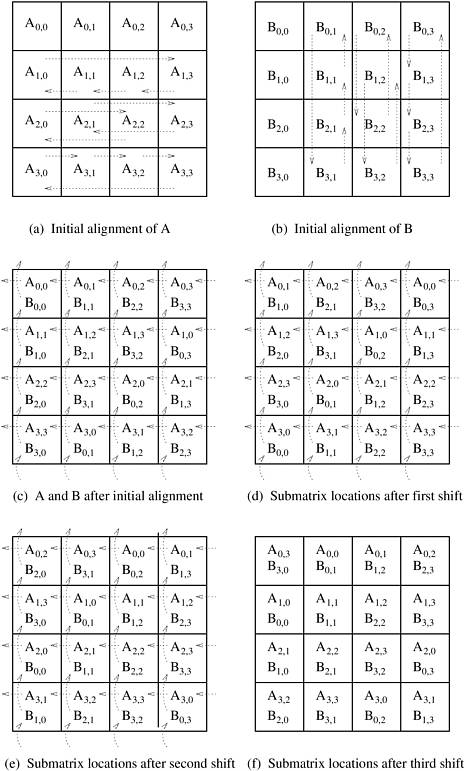
\includegraphics[scale=.5]{cannons}
\end{center}
\caption{Cannon's Algorithm}
\end{figure}

\subsection*{NumPy}

NumPy or \textit{Numerical Python} is a library for Python that adds supprt for large, multi-dimensional arrays and matrices, along with a lot of different hig-level mathematical functions to operate these array or matrices. NumPy uses C to make mathematical algorithms run much faster in Python, as this type of operations are much slower in Python than in the compiled language equivelent.

NumPy rewrites some Python code, mostly inner loops to achieve this.

\begin{figure}[H]
\begin{center}

\includegraphics[scale=.3]{numpy}
\end{center}
\caption{Numpy}
\end{figure}

NumPy's core functionality is \texit{ndarray} that stands for \textit{n}-dimensional array, data structure. NumPy's arrays have to be homogeneously typed (all the elements of a single array must be f the same type) while Python's arrays are rather lists or dynamic arrays, which means that is a mutable array that has random access, it has a variable size, and allows elements to be added or removed.

\section*{3. Implementation}

We will use Python and C for our implementation. We chose Python for its versatility, when it comes to work with files, executing system commands, etc. We chose C, as C being an compiling language makes it faster, this will help us speed up matrix multiplication in Python.

We started by implementing a straight forward matrix multiplication C code generator in Python. This script generated one line for each one of the variables of the resulting matrix, and it will fill up with the needed operations using for loops for writing the code. After generating the code, the script will compile and run the code. This script was our first implementation, and we used it as a first version on which we will work towards optimization.

As having to write, and then run all the values of the multiplication for each of the values of the result matrix, was computationally, and therefore time expensive, we decided to make few adjustments. What would make more sense is to first declare the values of the matrix, and then reference them inside a C loop for calculating the result matrix, so we changed the way we generated code and started by declaring all the values, and implemented some for loops in the C code. With this simple, yet important improvement, we managed to speed up our code. 

After some quick analisys to, we found out that the parts of the code generation tool that took most time were the part of compiling the code, and the code generation part in which we build the code. So we worked on this parts in our next iteration.

In the third iteration of our design, we decided to use a template instead of generating the code on the fly, this should help reduce the time, as it will use a template, and replace some of its parts, with the ones specific to each problem, rather than generate the whole code every time we run the script. We first created the template, and defined some lines in which we will introduce our code, then we used regular expressions to find the line that we wanted to replace with values specific to our problem. After that we will save the template with the replaced values, compile and run it. We also decided to use \textit{Tiny C Compiler} instead of \textit{GNU Compiler Collection}, to see if this lighter compiler will help us reduce the exponentially increasing compilation time of the generated code.

Then we compared both versions to see if this tweaks helped us to increase the performance of our code generation tool.


\begin{figure}[H]
\begin{center}
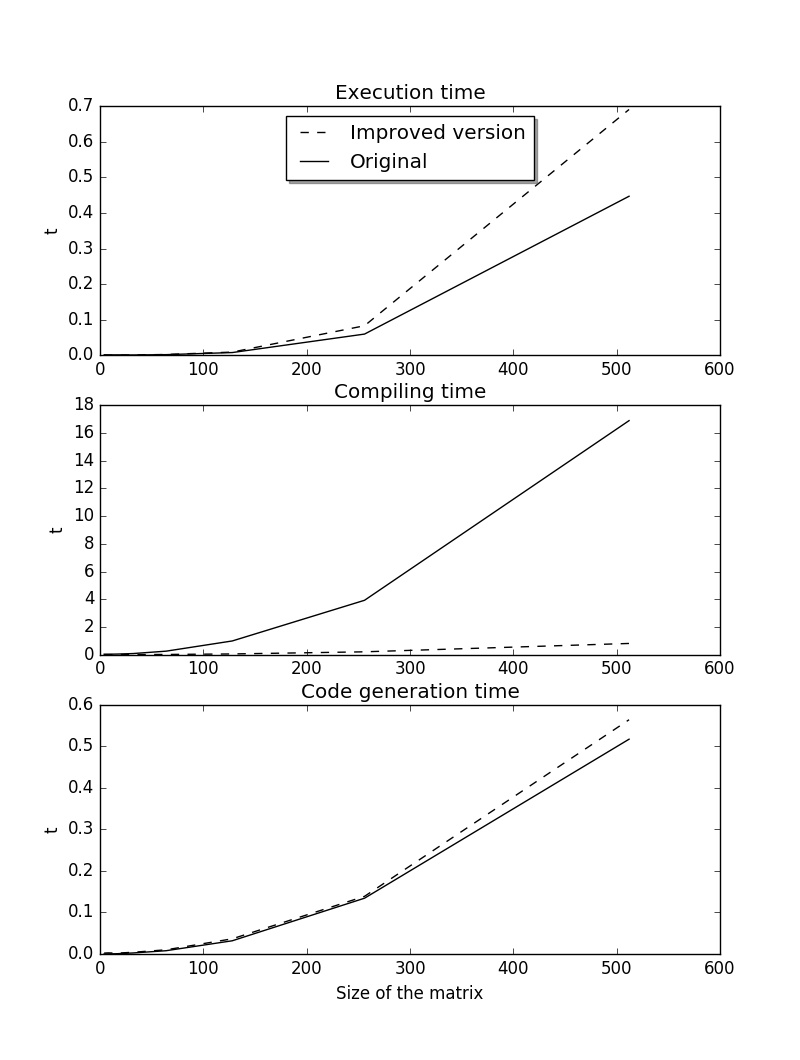
\includegraphics[scale=.2]{Plot}
\end{center}
\caption{Comparison between our two serial mult. implementations}
\end{figure}

As we can see in the results above, the new compiling time using the Tiny C Compiler is much smaller than the one using the GNU C Compiler, the onl downside of using Tiny Compiler is the increasing of running time, but the running time grows in a smaller rate than the decreasing rate of the compilation time, so we will use this compiler. We also found out that the new way of generating the code was slower than the one we had before, so we decided to stick to the code generator on the fly instead of using a template for our latest version.

Then we started implementing parallel marix multiplication. We tried two different implementations. One implementation calculates the result matrix by sending the full matrix to every node, then dividing the matrix, and calculate the matrix in parallel using \textbf{OpenMP}.

The other implementation will use Cannon's Algorithm for calculating the result matrix. In this case, the matrix will be divided into small submatrices, and one of this submatrices will be sent to each node. Then the nodes will comunicate between them to calculate the result matrix using \textbf{MPI}.

\section*{4. Experimental Work and Results}

Here we should talk about our algorithm complexity and how it scales. We can change the size of the matrices to see how it affects the performance. We should compare our implementation with tools like NumPy.

\section*{5. Conclusion and future work}

In this project, we approached different implementations for matrix multiplication, from serial matrix implementation to parallel matrix multiplication. We iterated over our initial design to improve our implementation's performance, which we increased by introducing small tweaks. For the matrix parallel muliplication we tried two different implementations, one using \textit{OpenMP} and sending one matrix to each node, and another implementation based on Cannon's algorithm that will send small pieces of the matrices to each of the nodes, and then the nodes will work as a group comunnicating using \textit{MPI}.

\begin{thebibliography}{9}
\bibitem{Joze}
\textit{Automatic generation of finite-element code by simultaneous optimization of expression}. Joze Korelc, 1997

\bibitem{Salvatore}
\textit{Dense Matrix-Matrix Multiplication in Parallel}. Salvatore Orlando, 2006

\bibitem{NumPy}
\textit{The NumPy Array: A Structure for Efficient Numerical Computation}.  Stefan van der Walt, S. Chris Colbert, Gael Varoquaux, IEEE 2011

\end{thebibliography}

\end{document}
